\documentclass[journal,twocolumn]{IEEEtran}

\usepackage[utf8]{inputenc}
\usepackage{graphicx}
\usepackage{amssymb}
\usepackage{mathtools}
\usepackage{amsmath}
\providecommand{\pr}[1]{\ensuremath{\Pr\left(#1\right)}}
\providecommand{\cbrak}[1]{\ensuremath{\left\{#1\right\}}}

\title{Assignment 8}
\author{Gollapudi Sasank CS21BTECH11019}

\begin{document}
\maketitle
\section*{Question : }
A fair coin is tossed twice , and let the random variable $X$ represent the number of heads. Find $F_X(x)$ (Cummulative Distribution Function of X)
\section*{Solution : }
Let us denote Head by $H$ and tail by $T$. \\
Sample Space(S) = \{HH,HT,TH,TT\}.\\
$X$ : Number of heads obtained \\
\begin{align}
X(HH) = 2 \\
X(HT) = 1 \\
X(TH) = 1 \\
X(TT) = 0 \\
\end{align}
\begin{align}
\pr{X=0} = \frac{1}{4} \\
\pr{X=1} = \frac{1}{2} \\
\pr{X=2} = \frac{1}{4}
\end{align}
From the definition of Cummulative Distribution Function(CDF) of a random variable $X$ 
\begin{align}
F_X(x) = \pr{X \le x}
\end{align}
\begin{enumerate}
\item For $x<0 $ , $X \le x \Rightarrow X<0$
\begin{align}
F_X(x) &= \pr{X<0} \\
F_X(x) &= 0
\end{align}
\item For $0 \le x < 1 $ , $X \le x \Rightarrow X<1$
\begin{align}
F_X(x) &= \pr{X < 1} \\
F_X(x) &= \pr{X=0} \\
F_X(x) &= \frac{1}{4}
\end{align}
\item For $ 1 \le x < 2$ , $X \le x \Rightarrow X<2$
\begin{align}
F_X(x) &= \pr{X < 2} \\
F_X(x) &= \pr{X=0} + \pr{X=1}  \\
F_X(x) &= \frac{1}{4} + \frac{1}{2} \\
F_X(x) &= \frac{3}{4}  
\end{align}
\item For $ x \ge 2 $ , $X \le x \Rightarrow X<\infty$
\begin{align}
F_X(x) &= \pr{X=0} + \pr{X=1} + \pr{X=2} \\
F_X(x) &= \frac{1}{4} + \frac{1}{2} + \frac{1}{4} \\
F_X(x) &= 1
\end{align}
\end{enumerate}
\begin{figure}[h]
\centering
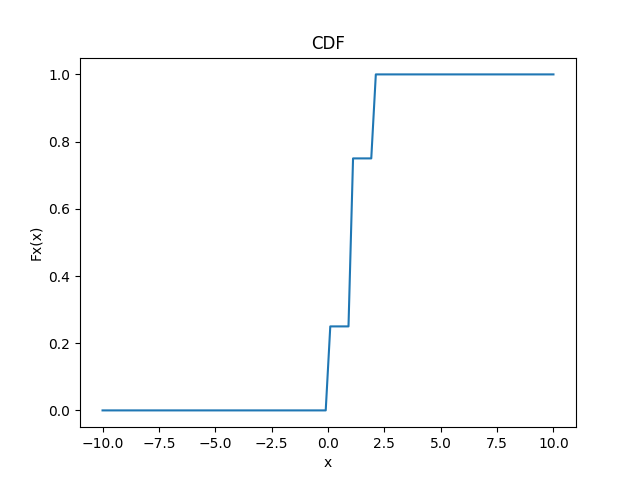
\includegraphics[width=\columnwidth]{Fig1.png}
\caption{CDF graph}
\label{Fig 1}
\end{figure}
\end{document}